\documentclass[a4paper]{article}
\usepackage[utf8]{inputenc}

% Author affiliation
\usepackage{authblk}
% Package for line spacing
\usepackage{setspace}
\renewcommand{\baselinestretch}{2.0} % Double spacing
% Margins
\usepackage[margin=1.25in]{geometry}
% Mathematics
\usepackage{amsmath}
% Tables
\usepackage{tabularx}
\usepackage{booktabs}
\usepackage{multirow}
\usepackage{makecell}
\usepackage{setspace}
% SI units
\usepackage{siunitx}
% Links and referencing within the document
\usepackage[backref]{hyperref}
\hypersetup{hidelinks} 
% Advanced math typesetting
\usepackage{mathtools}
% Graphics
\usepackage{graphicx}
\usepackage{subfig} 
\graphicspath{{./figures}} % Adjust path as needed

\title{An Example Test Document}

\author[1$\dag$]{Author A}
\author[1$\dag$]{Author B}
\author[1*]{Author C}
\author[1,2]{Author D}

\affil[1]{School of Example Studies, Example University}
\affil[2]{School of Advanced Example Studies, Example University}
\affil[*]{Address correspondence to: example.email@university.edu}
\affil[$\dag$]{These authors contributed equally to this work.}

\begin{document}

\maketitle

\begin{abstract}
This document provides a basic structure for an academic paper with test examples for tables, figures, formulas, and references. It includes examples of common LaTeX commands and document features.
\end{abstract}

\section{Introduction}

This document is a test example designed to help check various LaTeX formatting techniques, including tables, figures, and formulas. In the following sections, we will demonstrate these features.

\section{Tables}

There is a simple table in this section (Tab. \ref{tab:exampletable}).

\begin{table}[htbp]
    \centering
    \caption{
        An example table with parameters.
    }
    \label{tab:exampletable}
    \begin{tabular}{lcr}
        \toprule
        Parameter & Symbol & Value \\
        \midrule
        Example Parameter 1 & $P_1$ & \SI{100}{\watt} \\
        Example Parameter 2 & $P_2$ & \SI{50}{\meter} \\
        Example Parameter 3 & $P_3$ & \SI{0.1}{\second} \\
        \bottomrule
    \end{tabular}
\end{table}

Tab. \ref{table3} shows a more complex table.

\begin{table}[h]
    \begin{center}
        \begin{spacing}{1.15}
         \caption{Example Global Economic Indicators}\label{table3}
          \resizebox{0.85\hsize}{!}{
        \begin{tabular}{|c|c|c|}
            \hline
            \textbf{Region} & \textbf{Indicator} & \textbf{Value}  \\
            \hline

            \multirow{7}{*}{\makecell[{}{p{3cm}}]{Region A}} 
            & \multirow{3}{*}{\makecell[{}{p{3cm}}]{Economic Growth}} 
            & 3.5\%  \\
            \cline{3-3}
            &    & 1.5 trillion  \\
            \cline{3-3}
            &    & 4.8\% Inflation  \\
            \cline{2-3}

            & \multirow{4}{*}{\makecell[{}{p{3cm}}]{Unemployment Rate}}  
            & 5.1\%  \\
            \cline{3-3}
            &   & 2.4\% (Youth)  \\
            \cline{3-3}
            &   & 4.7\% (Women)  \\
            \cline{3-3}
            &   & 3.2\% (Men) \\
            \hline

            \multirow{6}{*}{\makecell[{}{p{3cm}}]{Region B}} 
            & \multirow{3}{*}{\makecell[{}{p{3cm}}]{Economic Growth}} 
            & 2.1\%  \\
            \cline{3-3}
            &    & 0.9 trillion  \\
            \cline{3-3}
            &    & 2.3\% Inflation  \\
            \cline{2-3}

            & \multirow{3}{*}{\makecell[{}{p{3cm}}]{Unemployment Rate}}  
            & 6.7\%  \\
            \cline{3-3}
            &   & 3.8\% (Youth)  \\
            \cline{3-3}
            &   & 4.5\% (Total)  \\
            \hline
        \end{tabular}
        }
        \end{spacing}
    \end{center}
\end{table}


\section{Figures and their References}

\subsection{Example Figure}

Below is an example figure (Fig. \ref{fig:examplefig}) showing a diagram that might represent a process or a conceptual flow.

\begin{figure}[htbp]
    \centering
    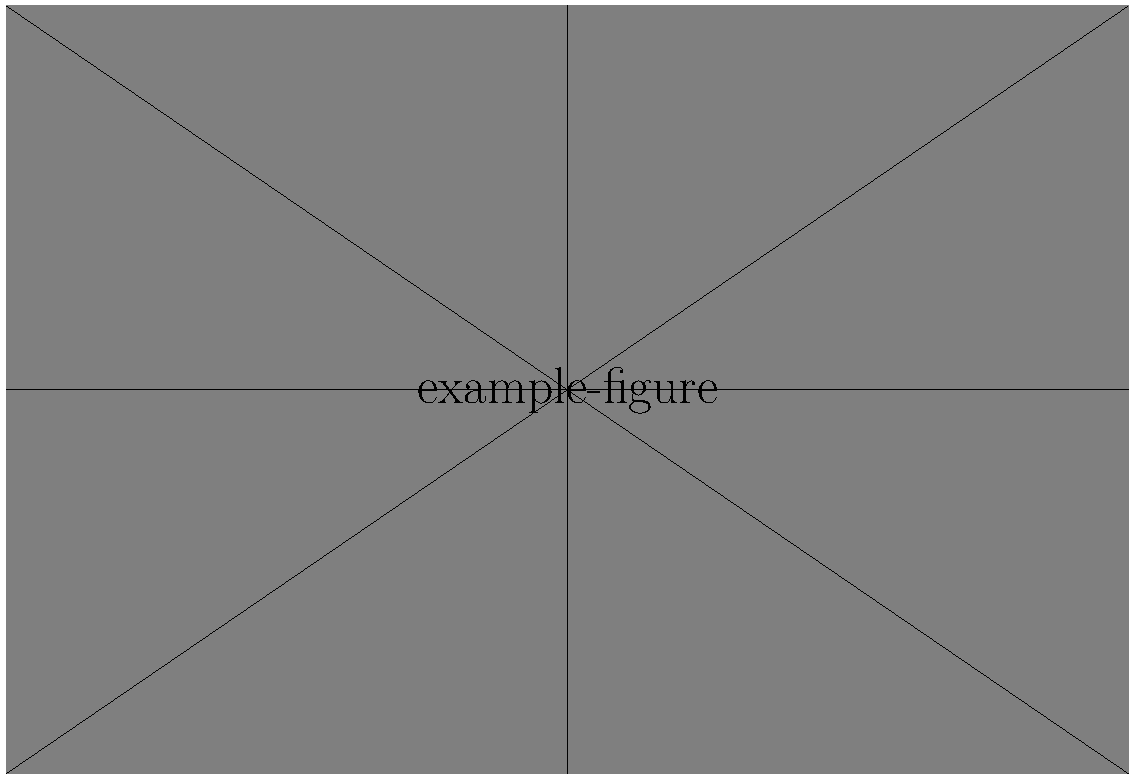
\includegraphics[width=0.8\linewidth]{example-figure}
    \caption{
        An example figure showing a conceptual diagram.
    }
    \label{fig:examplefig}
\end{figure}

\subsection{Subfigures}

Below is an example of subfigures (Fig. \ref{fig:examplesubfigures}), which contains 4 subfigures (Fig. \ref{fig:subfigure1}, Fig. \ref{fig:subfigure2}, Fig. \ref{fig:subfigure3}, and Fig. \ref{fig:subfigure4}).

\begin{figure}[htbp]
    \centering
    \subfloat[]{
        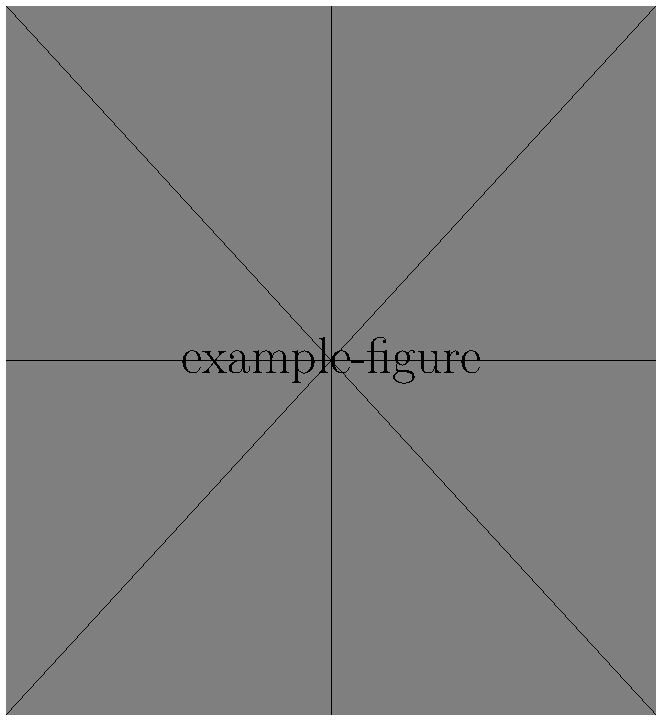
\includegraphics[width=0.31\linewidth]{example-subfigure1}\label{fig:subfigure1}
    }
    \subfloat[]{
        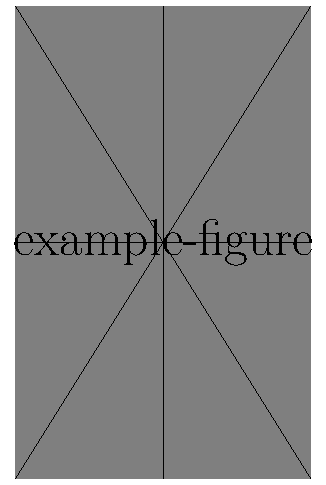
\includegraphics[width=0.23\linewidth]{example-subfigure2}\label{fig:subfigure2}
    }
    \subfloat[]{
        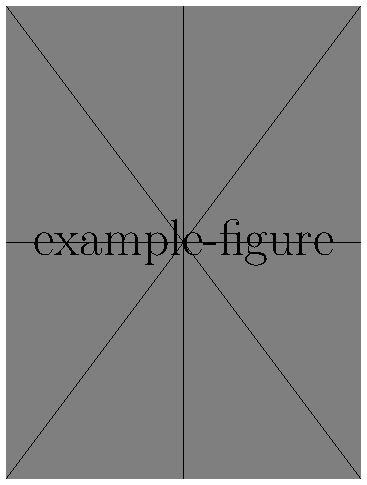
\includegraphics[width=0.24\linewidth]{example-subfigure3}\label{fig:subfigure3}
    }
    \\
    \subfloat[]{
        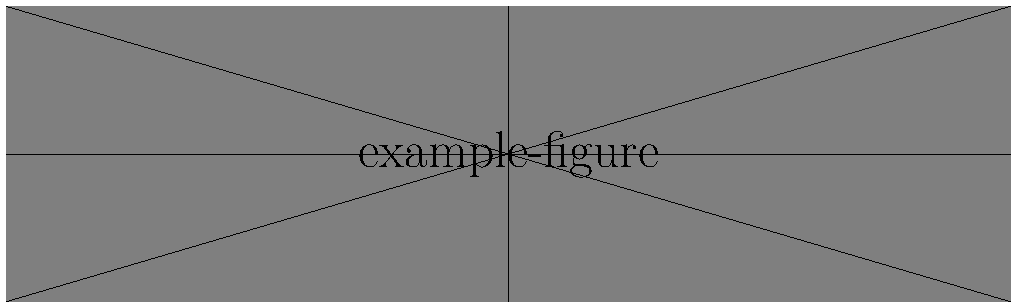
\includegraphics[width=0.8\linewidth]{example-subfigure4}\label{fig:subfigure4}
    }
    \caption{
        Example subfigures (a) Subfigure 1, (b) Subfigure 2, (c) Subfigure 3, and (d) Subfigure 4.
    }
    \label{fig:examplesubfigures}
\end{figure}

\section{Formulas and Equations}

This section includes an example of how to format equations. The incidence matrix is given by Eq. \ref{eq:incidence}:

\begin{align}\label{eq:incidence}
    a_{kl}=
    \begin{cases}
        1,  & \text{edge $l$ leaves node $k$},\\
        -1, & \text{edge $l$ enters node $k$},\\
        0,  & \text{otherwise},
    \end{cases}
\end{align}
where $a_{kl}$ is the element of the incidence matrix, $k$ is the node index, and $l$ is the edge index.

\section{References}

This section includes an example of how to cite references\cite{article1}.

\bibliographystyle{ieeetr}
\bibliography{../ref}

\end{document}
